\input ../talk-header.tex
\title
{Machine Learning}
\subtitle{CARTs}

\begin{document}

\maketitle

\begin{frame}{Data Set for Quiz}
  \vspace{1cm}
\vbox{
\hfil 2019-03-16 \hspace{5mm} 81682.0 \\
\hfil 2019-03-18 \hspace{5mm} 81720.0\\
\hfil 2019-03-20 \hspace{5mm} 81760.0\\
\hfil 2019-03-24 \hspace{5mm} 81826.0\\
\hfil 2019-03-25 \hspace{5mm} 81844.0\\
\hfil 2019-03-26 \hspace{5mm} 81864.0\\
\hfil 2019-03-27 \hspace{5mm} 81881.0\\
\hfil 2019-03-28 \hspace{5mm} 81900.0\\
\hfil 2019-03-30 \hspace{5mm} 81933.0\\
\hfil 2019-04-03 \hspace{5mm} 82003.0\\
}
\end{frame}

%%%%%%%%%%%%%%%%%%%%%%%%%%%%%%%%%%%%%%%%%%%%%%%%%%%%%%%%%%%%%%%%%%%%%%
%%%%%%%%%%%%%%%%%%%%%%%%%%%%%%%%%%%%%%%%%%%%%%%%%%%%%%%%%%%%%%%%%%%%%%
%%%%%%%%%%%%%%%%%%%%%%%%%%%%%%%%%%%%%%%%%%%%%%%%%%%%%%%%%%%%%%%%%%%%%%

\begin{frame}
  \vphrase{Review}
\end{frame}

\begin{frame}{What is Machine Learning?}
  Learning is what we do when we can't explain how.
  \begin{itemize}
  \item Supervised
  \item Unsupervised
  \item Reinforcement
  \end{itemize}
\end{frame}

\begin{frame}{Lots of maths}
  We'll try to ignore it, but it's there\dots
  \begin{itemize}
  \item Vector spaces and linear algebra
  \item Probability
  \item Statistics
  \item Optimisation theory
  \item Differential calculus
  \end{itemize}
  The curse of dimensionality.
\end{frame}

\begin{frame}{Data Science}
  \begin{enumerate}
  \item Define the question of interest
  \item Get the data
  \item Clean the data
  \item Explore the data
  \item Fit statistical models
  \item Communicate the results
  \item Make your analysis reproducible
  \end{enumerate}
\end{frame}

\begin{frame}{Data}
  \only<1>{\vphrase{Observational vs experimental}}
  \only<2>{\vphrase{Anecdote: it doesn't accumulate to be data.}}
  \only<3>{\cimgh{bias-variance.png}}
  \only<4>{\vphrase{Features}}
  \only<5>{\vphrase{Feature Engineering}}
  \only<6>{\vphrase{One of $K$ = one-hot encoding}}
  \only<7>{\vphrase{Outliers: don't ignore them!}}
\end{frame}

\begin{frame}{Feature Engineering}
  \begin{enumerate}
  \item Brainstorm
  \item Pick some
  \item Make them
  \item Evaluate
  \item Repeat
  \end{enumerate}
\end{frame}

\begin{frame}{Easy Features}
  \only<1>{\phrase{Text}\vspace{1cm}
    \centerline{bag of words}}
  \only<2>{\phrase{Images}\vspace{1cm}
    \centerline{corners, edges, point matching}}
  \only<3>{\vphrase{We'll see more}}
\end{frame}

\begin{frame}{Linear Regression}
  \only<1>{
    \textbf{Problem:}  $\{(x_i, y_i)\}$.

    Given $x$, predict $\hat y$.

    Here $y$ is continuous.
  }

  \only<2>{ $x$: \textbf{explanatory} or \textbf{predictor} variable.

    $y$: \textbf{response} variable.

    \vspace{1cm}
    \purple{For some reason, we believe a linear model is a good idea.}
  }
  

\end{frame}

\begin{frame}{Residuals}
  What's left over.
  \only<1>{
    \vspace{1cm}
    \begin{displaymath}
      \text{data} = \text{fit} + \text{residual}      
    \end{displaymath}
  }
  \only<2>{
    \vspace{1cm}
    \begin{displaymath}
      y_i = \hat y_i + e_i
    \end{displaymath}
  }
  \only<3>{
    Goal: small residuals.

    \vspace{1cm}
    \begin{displaymath}
      \sum e_i^2
    \end{displaymath}
  }
\end{frame}

\begin{frame}{Logistic regression}
  \only<1>{\begin{bphrase}
      \begin{itemize}
      \item Binary output
      \item Classification
      \end{itemize}
    \end{bphrase}
  }
  \only<2>{\begin{itemize}
    \item Have: continuous and discrete inputs
    \item Want: class (0 or 1)
    \end{itemize}
  }
  \only<3>{Logistic (sigmoid, logit) function
    \begin{mphrase}
      g(z) = \frac{1}{1+e^{-z}}
    \end{mphrase}
  }
\end{frame}

\begin{frame}{One vs Rest, One vs One}
  \only<1>{
    What I described yesterday:
    \begin{itemize}
    \item OvR (OvA): compute $k$ classifiers
    \item OvO: compute $k(k-1)/2$ classifiers
    \end{itemize}

    The missing point: the classifiers give scores, not just in/out answers.
  }
  \only<2>{
    One vs Rest:

    Accept the judgement of the classifier with the highest score.
  }
  \only<3>{
    One vs One:

    Classifiers vote.  Accept the class that gets the most votes.
  }
  \only<3>{
    Advantage:  Reduces multi-class classification to single-class classification.

    Disadvantage:  Classifier scores aren't necessarily comparable.  For example, classes
    may have very different numbers of members.
  }
\end{frame}

\begin{frame}{Hyperparameters}
  \only<1>{
    \begin{itemize}
    \item The word hyperparameter is not well-defined.
    \item In most contexts, it is the parameters of the underlying distribution
    \item In training, we learn the parameters of the model
    \item We choose the hyperparameters to govern the training
    \item So we may want to experiment to learn the distribution
      parameters that best optimise our learned model's performance
    \end{itemize}
  }
\end{frame}

\begin{frame}{Testing}
  \begin{itemize}
  \item Set aside (partition) data for testing (e.g., 70\% / 30\%)
  \item Learn on training set, test on testing set
  \item When searching hyperparameters, set aside again (e.g., 60\% / 20\% / 20\%)
  \end{itemize}
\end{frame}

%%%%%%%%%%%%%%%%%%%%%%%%%%%%%%%%%%%%%%%%%%%%%%%%%%%%%%%%%%%%%%%%%%%%%%
%\talksection{Break}

\begin{frame}
  % https://www.pexels.com/photo/scenic-view-of-lake-against-cloudy-sky-246642/
  % https://static.pexels.com/photos/246642/pexels-photo-246642.jpeg
  % CC0 license
  \cimgwb{maybe-skye.jpg}
  \vspace{-9.7cm}
  \phrase{questions?\hspace{2.2cm}}
\end{frame}

%%%%%%%%%%%%%%%%%%%%%%%%%%%%%%%%%%%%%%%%%%%%%%%%%%%%%%%%%%%%%%%%%%%%%%
%%%%%%%%%%%%%%%%%%%%%%%%%%%%%%%%%%%%%%%%%%%%%%%%%%%%%%%%%%%%%%%%%%%%%%
%%%%%%%%%%%%%%%%%%%%%%%%%%%%%%%%%%%%%%%%%%%%%%%%%%%%%%%%%%%%%%%%%%%%%%

\begin{frame}{The simple explanation}
  \only<1>{
    \cimghh{zDBbD.png}
  }
  \only<2>{
    \cimghh{aLZlG.png}
  }
  \only<3>{
    \cimghh{kxWgh.png}
  }
  \only<4>{
    \cimghh{ePy4V.png}
  }
  \only<5>{
    \cimghh{BWYYZ.png}
  }
  \only<6>{
    \cimghh{R9967.png}
  }
  \only<7>{
    \cimghh{WuxyO.png}
  }
  \only<8>{
    \cimghh{gWdPX.png}
  }
  \prevwork{\url{copperking@reddit}}
  % https://www.reddit.com/r/MachineLearning/comments/15zrpp/please_explain_support_vector_machines_svm_like_i
\end{frame}

\begin{frame}
  \vphrase{video time}
\end{frame}

%%%%%%%%%%%%%%%%%%%%%%%%%%%%%%%%%%%%%%%%%%%%%%%%%%%%%%%%%%%%%%%%%%%%%%
%\talksection{Break}

\begin{frame}
  % https://www.pexels.com/photo/vintage-old-book-document-142/
  % https://static.pexels.com/photos/142/vintage-old-book-document.jpg
  % CC0 license
  \cimgwb{vintage-old-book-document.jpg}
  %\vspace{-9.7cm}
  \vspace{-4.8cm}
  \phrase{questions?\hspace{1.4cm}}
\end{frame}

%%%%%%%%%%%%%%%%%%%%%%%%%%%%%%%%%%%%%%%%%%%%%%%%%%%%%%%%%%%%%%%%%%%%%%
%%%%%%%%%%%%%%%%%%%%%%%%%%%%%%%%%%%%%%%%%%%%%%%%%%%%%%%%%%%%%%%%%%%%%%
%%%%%%%%%%%%%%%%%%%%%%%%%%%%%%%%%%%%%%%%%%%%%%%%%%%%%%%%%%%%%%%%%%%%%%


\begin{frame}{Decision Trees}
  \only<1>{
    % https://www.pexels.com/photo/blue-geeen-and-orange-parrot-37833/
    % https://static.pexels.com/photos/37833/rainbow-lorikeet-parrots-australia-rainbow-37833.jpeg
    % CC0 license
    \vspace{-2cm}
    \cimgwb{rainbow-lorikeet-parrots-australia-rainbow.jpg}
  }
  \only<2>{\centerline{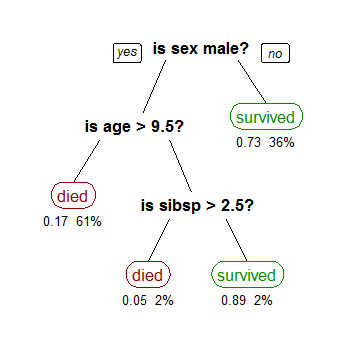
\includegraphics[height=.9\textheight]{tree_titanic_survivors.png}}
    % https://commons.wikimedia.org/wiki/File:CART_tree_titanic_survivors.png
    % License: CC ASA 3.0 unported.

    \vspace{-28mm}\parbox{.4\textwidth}{\red{E.g., passengers died
        with probability .17 which is 61\% of observations}}

    %\vspace{-18mm}
    \prevwork{Stephen Milborrow}
  }
\end{frame}

\begin{frame}{Quadtree}
  \cimgh{500px-Point_quadtree.png}
\end{frame}

\begin{frame}{$kd$-tree}
  \only<1>{
    \cimgh{370px-Kdtree_2d.png}
  }
  \only<2>{
    \cimgg{kd-tree-1.png}
  }
  \only<3>{
    \vphrase{$kd$-tree animation}
  }
\end{frame}

\begin{frame}{Decision Trees}
  \only<1>{
    Variations
    \begin{itemize}
    \item Classification tree
    \item Regression tree
    \end{itemize}
    \bigskip
    CART = classification and regression trees
  }
  \only<2>{
    % https://www.pexels.com/photo/nature-bird-australia-owl-105810/
    % https://static.pexels.com/photos/105810/pexels-photo-105810.jpeg
    % CC0 license
    \vspace{-3cm}
    \cimgwb{owl.jpg}
    \vspace{-8.7cm}
    \phrase{What can go wrong?}
  }
  \only<3>{
    Ensemble methods
    \begin{itemize}
    \item Bagging
    \item Random forest
    \item \gray{Boosted trees \textit{ (gradient boosted trees)}}
    \item \gray{Rotation forest}
    \end{itemize}
  }
\end{frame}

\begin{frame}{Boostrap aggregating = bagging}
  \only<1>{\phrase{Boostrap}

    A family of statistical methods using sampling with replacement.

    (Also: an example of an ensemble method.)
  }
  \only<2>{
    \begin{itemize}
    \item Increase stability
    \item Increase accuracy
    \item Reduce variance
    \item Avoid overfitting
    \end{itemize}
    A type of model averaging (ensemble method).
  }
  \only<3-4>{
    \begin{itemize}
    \item Training set $D$ of size $n$
    \item Sample $D$ \textit{with replacement} to create $D_1, \ldots, D_k$ of size $n'$
    \item If $n=n'$, expect $1-1/e \approx 63.2\%$ repeats
    \end{itemize}
  }
  \only<4>{
    \begin{itemize}
    \item Train $k$ models
    \item Average (regression) or vote (classification)
    \end{itemize}
  }
  \only<5>{
    Do not confuse with
    \begin{itemize}
    \item Boosting (and AdaBoost)
    \item Boostrap (statistics)
    \item Cross validation
    \end{itemize}
  }
\end{frame}

\begin{frame}{Random subspace method}
  \only<1>{
    \phrase{attribute bagging = feature bagging}
  }
  \only<2>{
    \blue{Bagging (bootstrap aggregation)} = resampling to create more
    data sets, train models on different samples

    \blue{Attribute bagging} = project to create more data sets, train
    models on different samples
  }
\end{frame}

\begin{frame}{Random forests}
  \only<1>{
    \vspace{1cm}
    \centerline{Combine \blue{bagging} with \blue{random subspace method}}
  }
\end{frame}

\begin{frame}{scikit-learn}
  \vspace{1cm}
  \vbox{\tt
    from sklearn.ensemble import RandomForestClassifier\\[5mm]

    X = [[0, 0], [1, 1]]\\
    Y = [0, 1]\\
    clf = RandomForestClassifier(n\_estimators=10)\\
    clf = clf.fit(X, Y)\\
    clf.predict([[.6, .6]])
  }

  \only<2>{
    \vspace{5mm}
    \purple{\texttt{X} has size \texttt{[n\_samples, n\_features]}}
    
    \purple{\texttt{Y} has size \texttt{[n\_samples]}}
  }
\end{frame}

\begin{frame}{scikit-learn}
  \vspace{1cm}
  \vbox{\tt
    from sklearn.ensemble import RandomForestRegressor\\[5mm]

    X = [[0, 0], [1, 1]]\\
    Y = [0, 1]\\
    clf = RandomForestRegressor(n\_estimators=10)\\
    clf = clf.fit(X, Y)\\
    clf.predict([[.6, .6]])
  }

  \only<2>{
    \vspace{5mm}
    \purple{\texttt{X} has size \texttt{[n\_samples, n\_features]}}
    
    \purple{\texttt{Y} has size \texttt{[n\_samples]}}
  }
\end{frame}

%%%%%%%%%%%%%%%%%%%%%%%%%%%%%%%%%%%%%%%%%%%%%%%%%%%%%%%%%%%%%%%%%%%%%%
%\talksection{Break}

\begin{frame}
  % https://www.pexels.com/photo/branches-fog-forest-landscape-235635/
  % https://static.pexels.com/photos/235635/pexels-photo-235635.jpeg
  % CC0 license
  \cimgwb{forest.jpg}
  \vspace{-9cm}
  \phrase{questions?}
\end{frame}


\end{document}
